\chapter{Design}
\label{cha:design}

As detailed in the previous chapters, the Spoofax language workbench already
offers a wide variety of services to assist in developing new domain specific
language. However, not all exposed functionality can be easily used from within
the context of a REPL, where a user just wants to be able to type in some text
and see a result.

An example is the various transformation goals made available to the user by a
language designer. There is no such thing as a uniform 'evaluation command',
that works across all languages, but instead each language defines its own
transform goals, of which one is an evaluation goal.  Furthermore the sequence
of processing steps needed to go from source to parsed source and transformed
result also varies between languages. One of the main goals the design had to
accomplish was therefore to expose a uniform interface for the various
transformation stages to REPL clients.

In \cref{sec:overview} an overview of the product design and its various
components will be given first. Afterwards the individual components will be
explained in more depth. In \cref{sec:commands} it will be addressed how a
uniform interface is presented to clients by encapsulating operations in
commands. In \cref{sec:function-comp} we will detail how commands have been
decomposed into smaller functions, which allows clients to build their own
transformation pipeline. \cref{sec:visitor} will then explain how this
transformation result is returned to the REPL client.

Finally, in \cref{sec:eval-strat}, the Dynsem evaluation strategy will be
outlined.  Afterwards it will be explained how other evaluation strategies
could be added to the existing design to support other interpreter backends,
such as Stratego. \cref{sec:eval-strat} then concludes with an overview of the changes
a language designer should make to its syntax and semantics to accomodate a
fully functioning REPL.

\section{Overview}
\label{sec:overview}


\begin{figure}[h]
  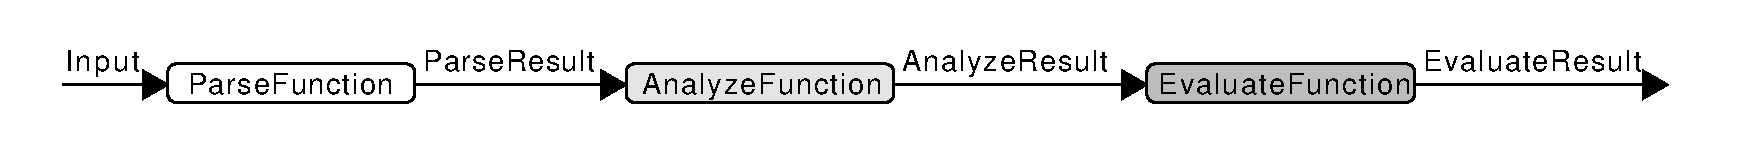
\includegraphics[width=\textwidth]{unit-flow}
  \caption{Processing steps for a language }
\end{figure}

\section{}
\label{sec:commands}

\begin{figure}[h]
  \centering
  \includegraphics[width=\textwidth]{uml-commands}
  \caption{UML of the various commands clients can execute.}
\end{figure}

\section{}
\label{sec:function-comp}

\section{}
\label{sec:visitor}

\section{}
\label{sec:eval-strat}

%%% Local Variables:
%%% mode: latex
%%% TeX-master: "main"
%%% End:
